The purpose of this documentation is to provide future developers a
roadmap of the most important parts of the Galant implementation. These can
be divided into several main aspects of Galant functionality:
\begin{itemize}
\item algorithm execution (Section~\ref{sec:execution})
\item macro expansion and compilation (Section~\ref{sec:compilation})
\item text editing and file management (Section~\ref{sec:editing})
\item graph editing and the graph window (Section~\ref{sec:graph_window})
\end{itemize}
In each case we consider sequences of events that take place as the result of
specific user or software actions, pointing out Java classes and methods that
handle the relevant functionality.

\section{Algorithm Execution} \label{sec:execution}

Algorithm execution is initiated when the user presses the \Code{Run} or
the \Code{Compile and Run} button when focused on an algorithm in the text
window. The sequence of method calls is
\begin{itemize}
\item \Code{run()} in \Code{gui.editor.GAlgorithmEditorPanel}; this
  initializes the current algorithm, the graph on which it will be run and
  the \Code{AlgorithmSynchronizer} and \Code{AlgorithmExecutor} that will be
  used to coordinate the algorithm with the GUI, respectively.

  The \Code{AlgorithmExecutor} manages the master thread, i.e., the one
  associated with the gui, and the \Code{AlgorithmSynchronizer} manages the
  slave thread, the one executing the algorithm on behalf of the user.

\item Method \Code{startAlgorithm()} in \Code{algorithm.AlgorithmExecuter}
  is called to fire up the algorithm (slave).

  At this point the gui and the algorithm behave as coroutines. The gui cedes
  control to the algorithm in
  \Code{algorithm.AlgorithmExecuter.incrementDisplayState()} and enters a
  busy-wait loop until the algorithm is done with a \emph{step} (clarified
  below) or it is terminated.

  The algorithm cedes control to the gui in
  \Code{algorithm.AlgorithmSynchronizer.pauseExecution}, where it either
  indicates that a step is finished (resulting in an exit from the busy-wait
  loop) or responds to a gui request to terminate
  the algorithm -- the gui has set \Code{terminated} -- by throwing a
  \Code{Terminate} pseudo-exception.
\end{itemize}

\begin{figure}
  \begin{center}
    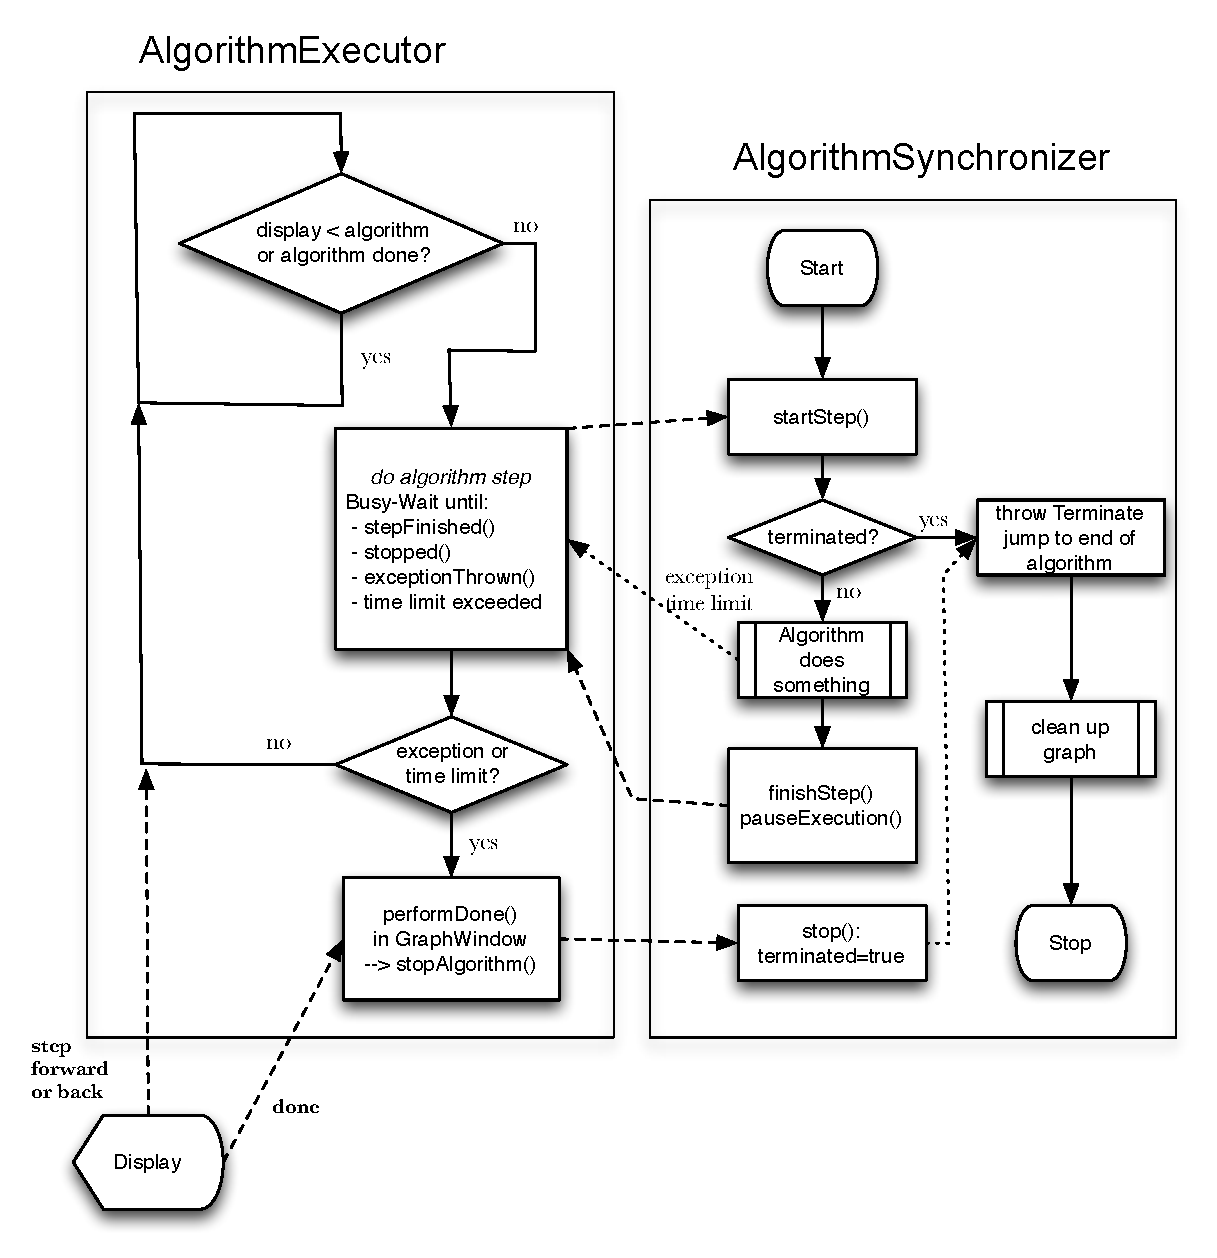
\includegraphics[width=\textwidth]{X-algorithm_execution}
  \end{center}
  \caption{Interactions between two threads during algorithm execution.}
  \label{fig:algorithm_execution}
\end{figure}

The gui controls algorithm execution, the user's view thereof, using the
buttons \Code{stepForward}, \Code{stepBackward} and \Code{done}, defined in
\Code{gui.window.GraphWindow}, or their keyboard shortcuts right arrow, left
arrow and escape, respectively.
Fig.~\ref{fig:algorithm_execution} gives a rough idea of the interaction
between the two threads (\Code{AlgorithmExecutor} and
\Code{AlgorithmSynchronizer}) that are active during algorithm execution.

\begin{itemize}
\item A step forward button press or arrow key effects a call to
  \Code{performStepForward()} in \Code{GraphWindow}, leading to an
  \Code{incrementDisplayState()}. First, there is a test,
  \Code{hasNextState()} in \Code{AlgorithmExecuter}, false only if the
  display shows the state of affairs after the algorithm has taken its last
  step.

\item \Code{incrementDisplayState()} does nothing (except increment the
  \Code{displayState} counter) if the algorithm execution is ahead of
  what the display shows (as a result of backward steps).

\item If the display state is current with respect to algorithm
  execution, the algorithm needs to execute another step -- the gui cedes
  control and enters its busy-wait loop. At this point the algorithm performs
  a step, described in more detail below.

\item A step back button press or array key effects a call to
  \Code{performStepBack()} in \Code{GraphWindow}, leading to a
  \Code{decrementDisplayState()}. The latter simply decrements the
  \Code{displayState} counter. If the display state corresponds to the
  beginning of algorithm execution -- \Code{hasPreviousState()} in
  \Code{AlgorithmExecutor} is false -- \Code{decrementDisplayState()} is not
  called.

\item The methods \Code{performStepForward()} and \Code{performStepBack()}
  also control the enabling and disabling of the corresponding buttons in the
  graph window, based on \Code{hasNextState()} and
  \Code{hasPreviousState()}. And they call \Code{updateStatusLabel()} to
  display the current algorithm and display states to the user. An algorithm
  state corresponds to a step in the algorithm.

\item A done button press or escape key leads to \Code{performDone()}, which
  in turn calls \Code{stopAlgorithm()} in the \Code{AlgorithmExecutor}.
  Here things get interesting. The \Code{AlgorithmSynchronizer} is told that
  the algorithm is to be stopped via a \Code{stop()} method call and the
  \Code{AlgorithmExecutor} cedes control to it. The algorithm is expected to
  yield control back to the executor, at which point the latter does a
  \Code{join()} to wait for the algorithm thread to finish. Algorithm and display
  states are then reinitialized to~0.

\item Complications arise with stopping the algorithm because the user may
  terminate the algorithm at any time, not just when the algorithm has run to
  completion. If it has not run to completion, the algorithm, at any
  attempt to execute the next step, checks whether it has been terminated. If so
  it throws \Code{Terminate}, an exception that is caught at the very end of
  the compiled algorithm. The effect is that of a ``long jump'' to the end of
  the algorithm.
\end{itemize}

Some complications that require extra care are:

\begin{itemize}
  \item The algorithm could throw an exception. If this is a
    \Code{GalantException} the constructor informs the
    \Code{AlgorithmSynchronizer} via a call to
    \Code{reportExceptionThrown()}.
    Other exceptions may cause Galant to hang. The ultimate goal is to avoid
    these entirely. In the \Code{Algorithm} class, which defines all the
    procedural-style method calls, potential null pointer exceptions are
    caught before the underlying graph methods are called.
\end{itemize}


% [Last modified: 2016 12 05 at 22:21:12 GMT]
